\documentclass[lettersize,journal]{IEEEtran}
\usepackage{amsmath,amsfonts}
\usepackage{algorithmic}
\usepackage{algorithm}
\usepackage{array}
\usepackage[caption=false,font=normalsize,labelfont=sf,textfont=sf]{subfig}
\usepackage{textcomp}
\usepackage{stfloats}
\usepackage{url}
\usepackage{verbatim}
\usepackage{graphicx}
\usepackage{cite}
\hyphenation{op-tical net-works semi-conduc-tor IEEE-Xplore}

\begin{document}

\title{NEURAL NETWORKS - DEEP LEARNING \\ SECOND ASSIGNMENT}

\author{Dimitrios Diakoloukas 10642, Electrical and Computer Engineering,~\IEEEmembership {AUTH, Student}

\thanks{}
\thanks{}}

% The paper headers
\markboth{SECOND ASSIGNMENT NEURAL NETWORKS - DEEP LEARNING, 
 November~2024}%
{Shell \MakeLowercase{\textit{et al.}}: A Sample Article Using IEEEtran.cls for IEEE Journals}

\maketitle

\begin{abstract}
This study presents the implementation of multiple Support Vector Machines (SVMs) for multi-class image classification on the CIFAR-10 dataset. The CIFAR-10 dataset, using 60,000 images across 10 categories, was preprocessed using Principal Component Analysis (PCA) to reduce dimensionality while preserving 90\% of the data's variability. The SVM models were then trained and evaluated, often employing cross-validation to ensure robust performance. 
To assess the model's efficacy, classification metrics such as accuracy, confusion matrices, and precision-recall curves were analyzed. Additionally, comparisons were made with other classifiers, including \textit{k}-Nearest Neighbors (\textit{k}-NN) and a Multi-Layer Perceptron (MLP). This study highlights the effectiveness of SVMs in image classification tasks and explores the influence of hyperparameter tuning and loss functions on model performance.
\end{abstract}

\section{\textbf{Introduction}}
\IEEEPARstart{I}{mage} classification is an essential task in computer vision, used in areas like autonomous driving and facial recognition. The CIFAR-10 dataset, a widely recognized dataset, presents us with the problem of classifying images into 10 distinct categories, each of which has natural objects such as animals and vehicles. Support Vector Machines (SVMs), known for their strong theoretical foundations and versatility, are commonly applied to such tasks because of their ability to handle high-dimensional data effectively. The main point of this assignment is to further experiment with SVMs.

\section{\textbf{Data Loading and Preprocessing}}

This section explains how I loaded the CIFAR-10 dataset and prepared it so that it could be used with the SVM implementations but also (\textit{k}-NN) algorithm and MLP implementation for testing purposes.

\subsection{\textbf{Loading CIFAR-10 Data}}
The CIFAR-10 dataset contains 60,000 small color images (32x32 pixels) across 10 different classes. There are 50,000 images for training and 10,000 images for testing. Each image is stored as a set of pixel values and the data is divided into multiple files.

I used the following steps to load the data:
\begin{itemize}
    \item \textbf{Unpacking Data Files:} The training data is stored in five files, each containing 10,000 images. I created a helper function called unpickle to open each file and load the data inside.
    \item \textbf{Combining Training Files:} I combined the data from all five training files into one large set. This gave us a total of 50,000 images for training. I did the same for the labels, so each image has a label showing which class it belongs to.
    \item \textbf{Loading Test Data:} The test data is stored in a separate file. I loaded this file in the same way to get 10,000 test images and their labels.
\end{itemize}

\subsection{\textbf{Data Preprocessing}}
After loading the data, I prepared it for use with machine learning by following these steps:

\begin{itemize}
    \item \textbf{Reshaping Images:} Each image was originally stored as a long row of numbers (a flat array). I reshaped these numbers back into the original 32x32 size with 3 color channels (Red, Green, and Blue).
    \item \textbf{Normalizing Pixel Values:} The pixel values in each image were originally between 0 and 255. To make the data easier to work with, I scaled these values to be between 0 and 1 by dividing each value by 255. This helps the model perform better and faster.
\end{itemize}

The final output of our data loading and preprocessing is:
\begin{itemize}
    \item \texttt{x\_train}: A set of 50,000 training images, each with shape (32, 32, 3) and pixel values between 0 and 1.
    \item \texttt{y\_train}: A set of 50,000 labels for the training images.
    \item \texttt{x\_test}: A set of 10,000 test images, also with shape (32, 32, 3) and pixel values between 0 and 1.
    \item \texttt{y\_test}: A set of 10,000 labels for the test images.
\end{itemize}
\vspace{0.3cm}
This data is now ready to be used in our CNN and MLP algorithms as well as the k-NN algorithm, making it easy to classify each image based on its pixel values.

\section{\textbf{Differences Between Linear, Sigmoid, RBF, and Polynomial Kernels}}

Kernels are functions used in machine learning, especially in Support Vector Machines (SVMs), to transform data into a higher-dimensional space where it may become linearly separable. Below, I describe the differences between the linear, sigmoid, radial basis function (RBF), and polynomial kernels:

\subsection{\textbf{Linear Kernel}}
The linear kernel is the simplest kernel function and is defined as:
\[
K(\mathbf{x}_i, \mathbf{x}_j) = \mathbf{x}_i^\top \mathbf{x}_j
\]
- \textbf{Usage:} It is used when the data is linearly separable.

\vspace{0.1cm}

\hspace{-0.33cm}- \textbf{Advantages:} Computationally efficient and interpretable.

\vspace{0.1cm}

\hspace{-0.33cm}- \textbf{Disadvantages:} Limited to linearly separable problems.

\subsection{\textbf{Sigmoid Kernel}}
The sigmoid kernel is defined as:
\[
K(\mathbf{x}_i, \mathbf{x}_j) = \tanh(\gamma \mathbf{x}_i^\top \mathbf{x}_j + r)
\]
Where:
\begin{itemize}
    \item $\gamma$ is a scaling parameter.
    \item $r$ is a shift parameter.
\end{itemize}
- \textbf{Usage:} It is inspired by neural networks and mimics their activation function.

\vspace{0.1cm}

\hspace{-0.33cm}- \textbf{Advantages:} Suitable for specific tasks involving non-linear data.

\vspace{0.1cm}

\hspace{-0.33cm}- \textbf{Disadvantages:} Its performance can be sensitive to parameter choices, and it may not be positive semi-definite for all values of $\gamma$ and $r$.

\subsection{\textbf{Radial Basis Function (RBF) Kernel}}
The RBF kernel, also known as the Gaussian kernel, is given by:
\[
K(\mathbf{x}_i, \mathbf{x}_j) = \exp\left(-\gamma \|\mathbf{x}_i - \mathbf{x}_j\|^2\right)
\]
Where $\gamma > 0$ controls the spread of the kernel.
- \textbf{Usage:} It is highly effective in cases of non-linearly separable data.

\vspace{0.1cm}

\hspace{-0.33cm}- \textbf{Advantages:} It can map input data into an infinite-dimensional space and is widely used for non-linear problems.

\vspace{0.1cm}

\hspace{-0.33cm}- \textbf{Disadvantages:} Requires careful tuning of $\gamma$ to prevent overfitting or underfitting.

\subsection{\textbf{Polynomial Kernel}}
The polynomial kernel is defined as:
\[
K(\mathbf{x}_i, \mathbf{x}_j) = (\gamma \mathbf{x}_i^\top \mathbf{x}_j + r)^d
\]
Where:
\begin{itemize}
    \item $\gamma$ is a scaling parameter.
    \item $r$ is a shift parameter.
    \item $d$ is the degree of the polynomial.
\end{itemize}
- \textbf{Usage:} Suitable for capturing complex non-linear relationships.

\vspace{0.1cm}

\hspace{-0.33cm}- \textbf{Advantages:} Capable of representing intricate structures in data.

\vspace{0.1cm}

\hspace{-0.33cm}- \textbf{Disadvantages:} High degree polynomials can lead to overfitting, and computational cost increases with $d$.

\subsection{\textbf{Summary Table}}
\begin{center}
\begin{tabular}{|m{0.12\textwidth}|>{\centering\arraybackslash}m{0.16\textwidth}|m{0.13\textwidth}|}
\hline
\textbf{Kernel} & \textbf{Expression} & \textbf{Key Features} \\
\hline
Linear & $\mathbf{x}_i^\top \mathbf{x}_j$ & For linearly separable data. \\
\hline
Sigmoid & $\tanh(\gamma \mathbf{x}_i^\top \mathbf{x}_j + r)$ & Mimics neural network activation functions. \\
\hline
RBF & $\exp\left(-\gamma \|\mathbf{x}_i - \mathbf{x}_j\|^2\right)$ & Excellent for non-linear problems. \\
\hline
Polynomial & $(\gamma \mathbf{x}_i^\top \mathbf{x}_j + r)^d$ & Captures complex non-linear structures. \\
\hline
\end{tabular}
\end{center}

\vspace{0.5cm}

\section{\textbf{SVM Using LIBSVM: Analysis without and with PCA}}
In this section, we applied Support Vector Machines (SVM) using the LIBSVM library to classify images from the CIFAR-10 dataset, but did not apply grid search techniques for hyperparameter tuning.

\subsection{\textbf{No PCA Implementation Explanation}}
In the initial implementation without PCA to simplify the task, we selected two classes (label 0 and label 1) and performed binary classification.  The key steps involved were:

\begin{itemize}
    \item \textbf{Data Preparation}: Images from the two selected classes were reshaped and filtered. The dataset was split into 60\% for training and 40\% for testing. We also used 10000 samples instead of 60000 that the dataset has originally since without PCA the implementation took a long long time to finish.
    \item \textbf{Training SVM Models}: Using LIBSVM, we trained SVM models with four different kernel types: Linear, Polynomial, Radial Basis Function (RBF), and Sigmoid. Each kernel was tested to observe its performance.
    \item \textbf{Performance Evaluation}: The models were evaluated using metrics such as accuracy, confusion matrices, and classification reports. Additionally, the training and evaluation times were recorded.
\end{itemize}

\vspace{0.5cm}

\subsubsection{\textbf{Results and Observations}}
The SVM models were evaluated using four different kernels, and their performance is summarized below:

1. \textbf{Linear Kernel:}  
   The linear kernel had the longest training time (50.81 seconds) and achieved an accuracy of 77.10\%. Precision and recall were balanced for both classes, but it struggled to capture non-linear relationships in the data.

2. \textbf{Polynomial Kernel:}  
   The polynomial kernel trained faster (40.07 seconds) but had a slightly lower accuracy of 75.90\%. While it showed high precision for Class 0, its recall was low, indicating difficulty in correctly identifying all samples from Class 0. The overall performance was inconsistent.

3. \textbf{Radial Basis Function (RBF) Kernel:}  
   The RBF kernel had the shortest training time (31.30 seconds) and achieved the best accuracy of 81.37\%. Precision and recall were well-balanced, making it the most effective kernel for this task.

4. \textbf{Sigmoid Kernel:}  
   The sigmoid kernel's training and evaluation times were slightly longer than those of the RBF kernel, and its accuracy was 78.60\%. While its performance was better than the polynomial kernel, it was slightly weaker than the RBF kernel.

\vspace{0.3cm}
The implementation in Python for this is provided in the \texttt{svm\_libsvm\_no\_pca.py} file, and the results are stored in the \texttt{svm\_results\_2\_classes.txt} file.

Below are some confusion matrices showing the performance of the SVM model for different kernels. Each matrix represents the distribution of true labels versus predicted labels, highlighting the accuracy for each kernel:
\begin{figure}[H]
    \centering
    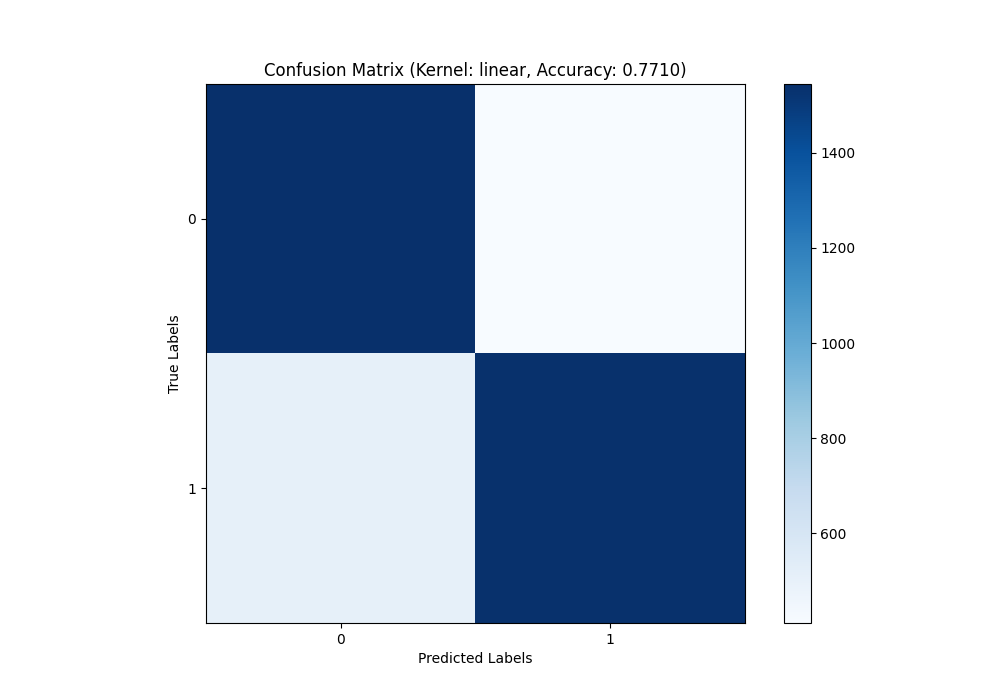
\includegraphics[width=0.5\textwidth]{confusion_matrix_2_classes_linear.png}
    \caption{Confusion Matrix for Linear Kernel.}
    \label{fig:confusion-matrix-linear}
\end{figure}
\begin{figure}[H]
    \centering
    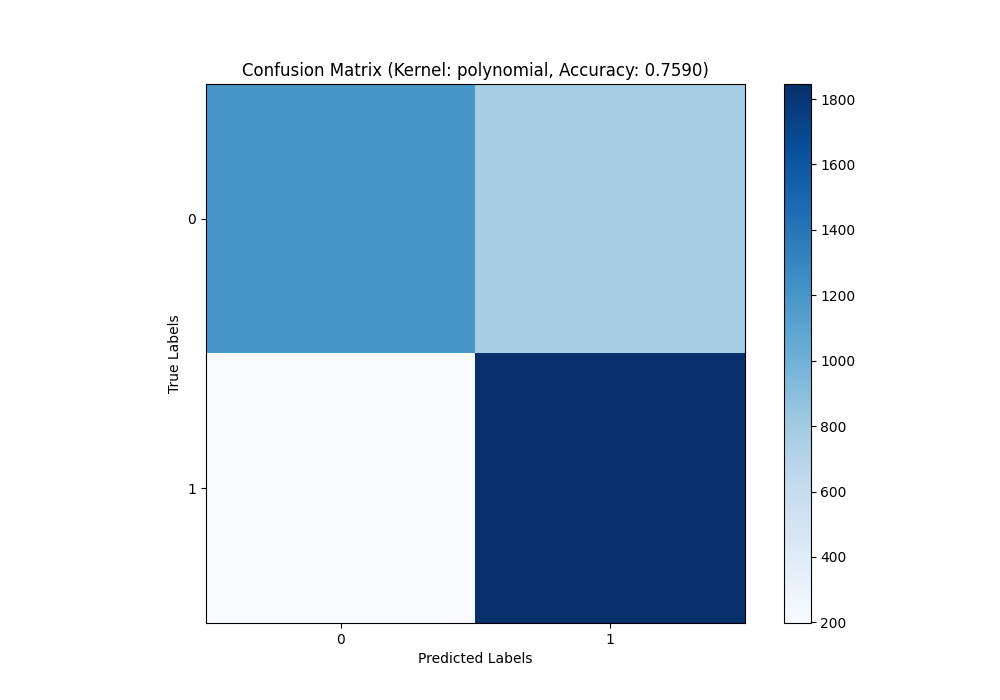
\includegraphics[width=0.5\textwidth]{confusion_matrix_2_classes_polynomial.png}
    \caption{Confusion Matrix for Polynomial Kernel.}
    \label{fig:confusion-matrix-polynomial}
\end{figure}
\begin{figure}[H]
    \centering
    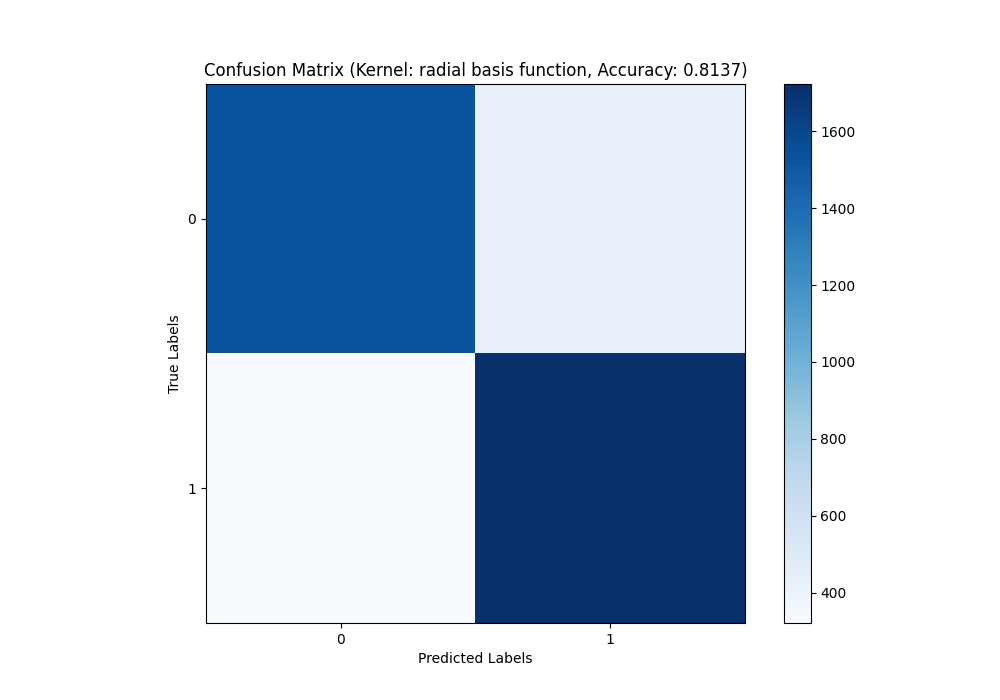
\includegraphics[width=0.5\textwidth]{confusion_matrix_2_classes_radial basis function.png}
    \caption{Confusion Matrix for RBF Kernel.}
    \label{fig:confusion-matrix-RBF}
\end{figure}
\begin{figure}[H]
    \centering
    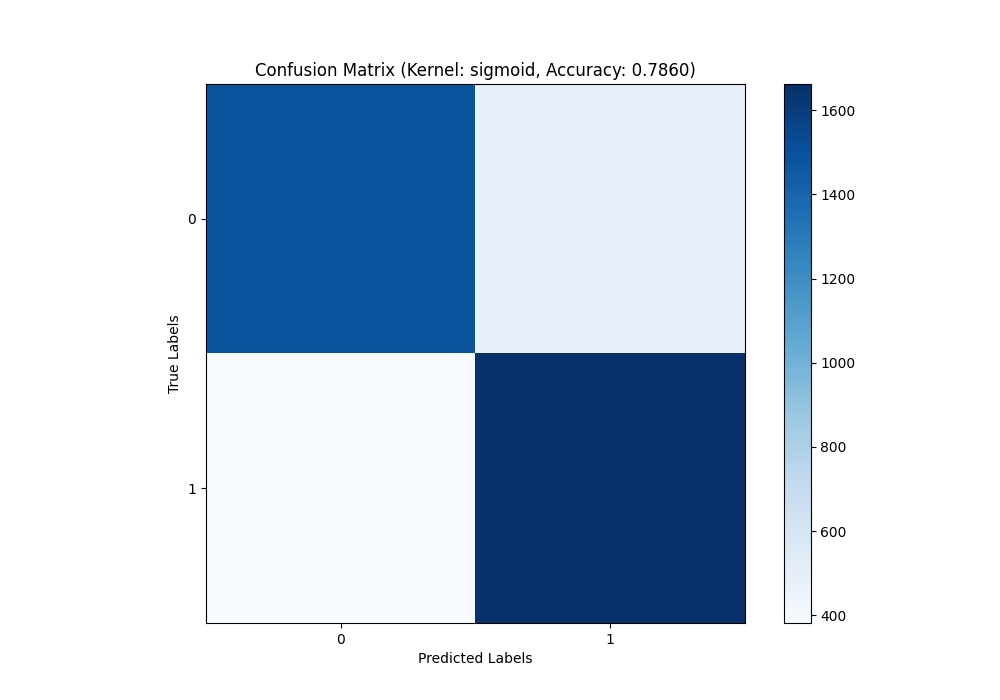
\includegraphics[width=0.5\textwidth]{confusion_matrix_2_classes_sigmoid.png}
    \caption{Confusion Matrix for Sigmoid Kernel.}
    \label{fig:confusion-matrix-sigmoid}
\end{figure}

\clearpage
\textbf{Conclusion:} The RBF kernel performed the best in terms of accuracy and balanced predictions. It is the most suitable kernel for this binary classification task, while the linear and polynomial kernels showed limitations in handling non-linear data.

\subsection{\textbf{PCA Implementation Explanation}}
To address the high dimensionality of the CIFAR-10 dataset and reduce computational complexity and be capable to use the entire 10 classes and 60000 sample dataset and finish training in a reasonable time, we implemented Principal Component Analysis (PCA). The key steps involved were:

\begin{itemize}
    \item \textbf{Dimensionality Reduction:} PCA was used to reduce the dataset's dimensionality while retaining 90\% of the original variance. This ensured that most of the critical information from the images was preserved.
    \item \textbf{Data Preparation:} After applying PCA, the dataset was split into 60\% for training and 40\% for testing. The reduced dataset allowed faster training and evaluation while still enabling meaningful performance comparisons.
    \item \textbf{Training SVM Models:} Similar to the no-PCA implementation, SVM models were trained using four kernel types: Linear, Polynomial, Radial Basis Function (RBF), and Sigmoid.
    \item \textbf{Performance Evaluation:} The models were evaluated using accuracy, confusion matrices, classification reports, and computation times.
\end{itemize}

\vspace{0.5cm}

\subsubsection{\textbf{Results and Observations}}
The results for the SVM models with PCA applied are summarized below:

1. \textbf{Linear Kernel:}  
   Training took 869.94 seconds, and the accuracy was 40.51\%. Precision and recall were low across all classes, indicating that the linear kernel struggled even with dimensionality reduction.

2. \textbf{Polynomial Kernel:}  
   Training time reduced significantly to 196.78 seconds, and accuracy improved to 46.25\%. Class-wise performance showed variability, with some classes achieving better precision and recall, but overall results were inconsistent.

3. \textbf{Radial Basis Function (RBF) Kernel:}  
   This kernel achieved the best accuracy of 53.29\% with a training time of 120.26 seconds. Precision and recall were more balanced across classes compared to other kernels, making it the most effective kernel even after PCA.

4. \textbf{Sigmoid Kernel:}  
   Despite the reduced training time of 70.17 seconds, accuracy dropped to 20.07\%. The sigmoid kernel performed poorly, with low precision and recall across all classes, suggesting that it was not suitable for this task.

\vspace{0.3cm}
The implementation in Python for this is provided in the \texttt{svm\_libsvm\_all.py} file, and the results are stored in the \texttt{svm\_results.txt} file.

Below are some confusion matrices showing the performance of the SVM model for different kernels after PCA. Each matrix highlights the predicted versus true labels and the corresponding accuracy.

\begin{figure}[H]
    \centering
    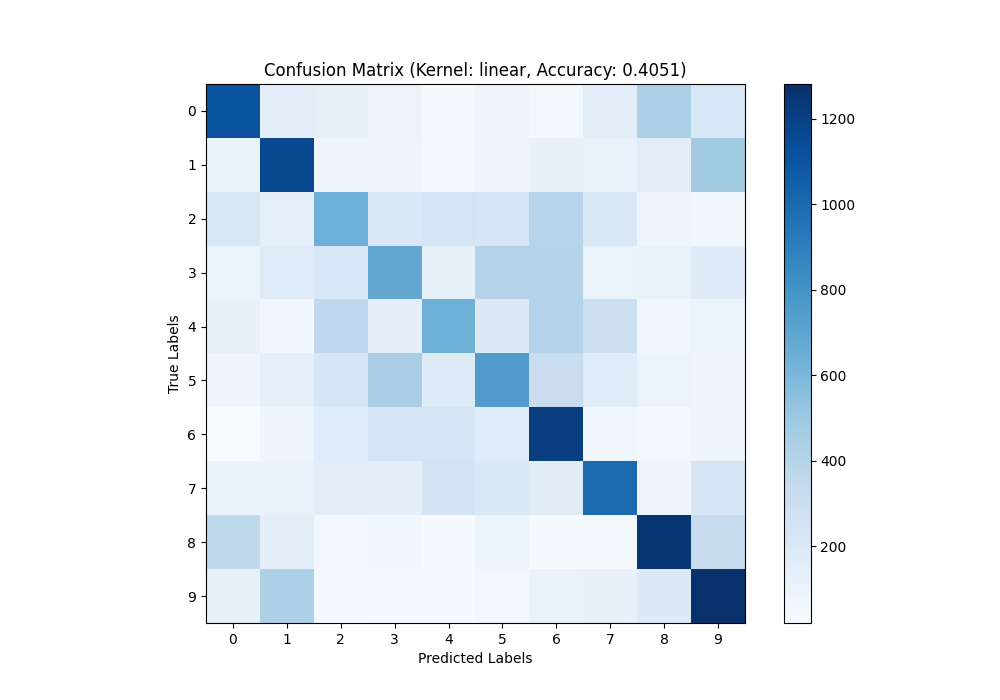
\includegraphics[width=0.5\textwidth]{confusion_matrix_linear.png}
    \caption{Confusion Matrix for Linear Kernel.}
    \label{fig:confusion-matrix-linear}
\end{figure}
\begin{figure}[H]
    \centering
    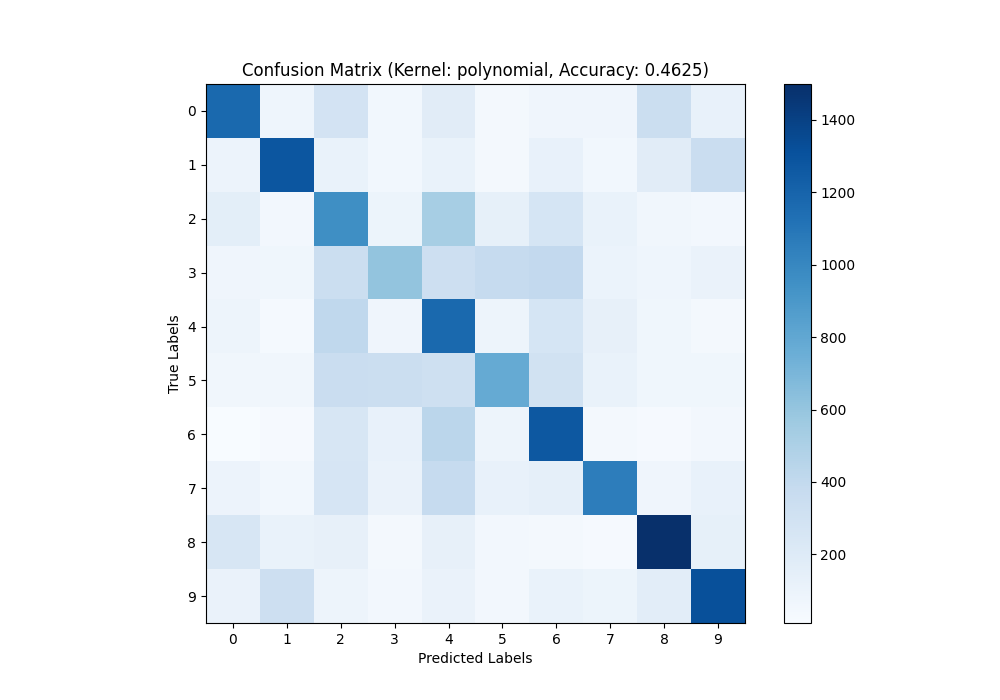
\includegraphics[width=0.5\textwidth]{confusion_matrix_polynomial.png}
    \caption{Confusion Matrix for Polynomial Kernel.}
    \label{fig:confusion-matrix-polynomial}
\end{figure}
\begin{figure}[H]
    \centering
    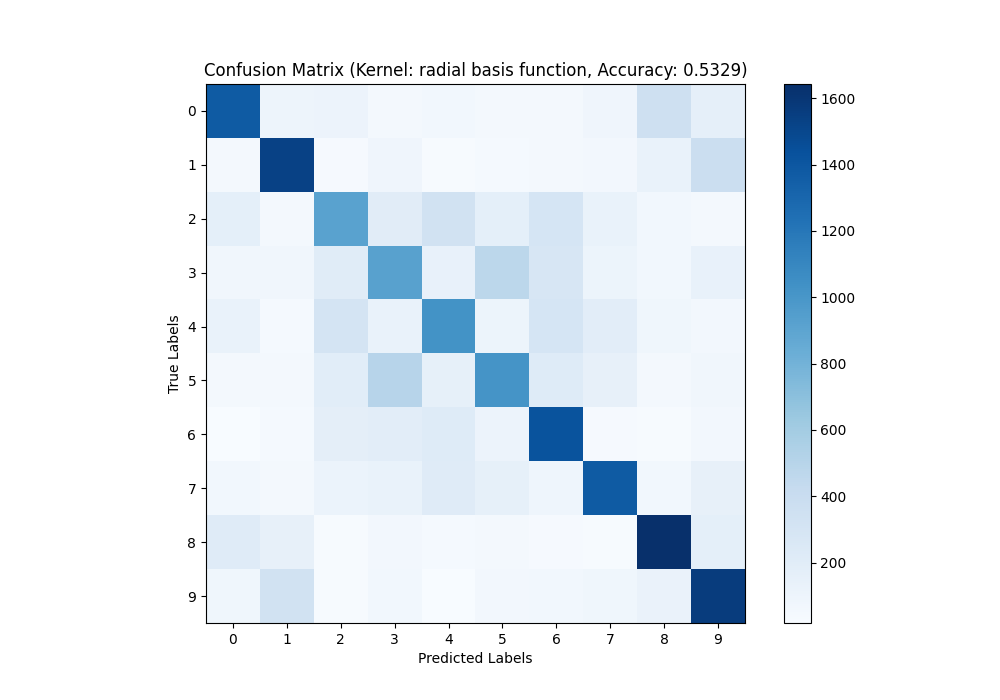
\includegraphics[width=0.5\textwidth]{confusion_matrix_radial basis function.png}
    \caption{Confusion Matrix for RBF Kernel.}
    \label{fig:confusion-matrix-RBF}
\end{figure}
\begin{figure}[H]
    \centering
    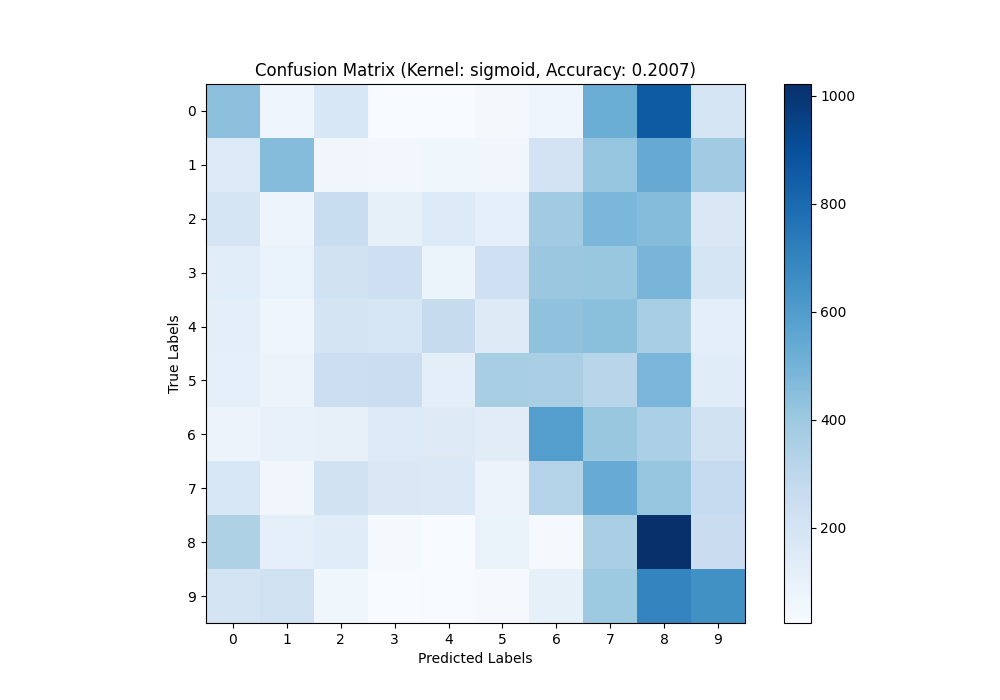
\includegraphics[width=0.5\textwidth]{confusion_matrix_sigmoid.png}
    \caption{Confusion Matrix for Sigmoid Kernel.}
    \label{fig:confusion-matrix-sigmoid}
\end{figure}

\textbf{Conclusion:}  
Applying PCA reduced the training and evaluation times significantly. However, while the RBF kernel maintained its superior performance, other kernels showed mixed results. The linear and sigmoid kernels performed poorly, while the polynomial kernel showed moderate improvement. Overall, PCA allowed faster training with some trade-offs in accuracy, particularly for simpler kernels.

This analysis allowed us to compare the performance of SVM models with and without PCA and across different kernels. The results, including accuracy and confusion matrices, clearly show the trade-offs of dimensionality reduction and kernel selection in image classification.

\section{\textbf{Grid Search Implementation Analysis}}

\subsection{\textbf{Grid Search Implementation}}
To find the best settings for SVM models, we used a method called grid search. This tested different kernel types (Linear, Polynomial, RBF, and Sigmoid) with combinations of regularization ($C$) and kernel ($\gamma$) parameters. Here’s how it was done:

\begin{itemize}
    \item \textbf{Parameter Testing:} We tested $C = \{0.1, 1, 10\}$ and $\gamma = \{0.001, 0.01, 0.1, 1\}$ for all kernels.
    \item \textbf{Kernel Types:} Different kernels were tried to check how well they could handle the data. These were Linear, Polynomial, RBF, and Sigmoid kernels.
    \item \textbf{Measuring Performance:} We checked how accurate the models were and used scores like precision, recall, and F1 to see how well they worked for different classes.
    \item \textbf{Training Time:} We recorded how long it took to train each model to compare their efficiency which will be demonstrated below. Although it is important to note that the training time for the grid search operation to select the best parameters took way to long specifically 16 hours and 21 minutes on my personal CPU.
\end{itemize}

\vspace{0.5cm}

\subsubsection{\textbf{Results and Observations}}
Here are the results for each kernel:

\begin{itemize}
    \item \textbf{Linear Kernel:}  
        
        - Training Time: 176.15 seconds 
        
        - Testing Accuracy: 40.54\%  
        
        - Observations: This kernel was simple and fast but couldn’t handle the complexity of the data well.

    \item \textbf{Polynomial Kernel:}  
        
        - Training Time: 258.34 seconds  
        
        - Testing Accuracy: 42.78\% 
        
        - Observations: The polynomial kernel did better than the linear one but took more time to train.

    \item \textbf{RBF Kernel:}  
        
        - Training Time: 256.84 seconds  
        
        - Testing Accuracy: 9.59\%  
        
        - Observations: The RBF kernel performed very poorly, likely because its settings were not suitable for the dataset. It seems like it has so low accuracy which is almost random guessing.

    \item \textbf{Sigmoid Kernel:}  
        
        - Training Time: 101.78 seconds  
        
        - Testing Accuracy: 38.16\%  
        
        - Observations: The sigmoid kernel was quick to train but didn’t give good results overall.

    \item \textbf{k-Nearest Neighbors (k-NN):}  
    
        - Testing Accuracy: 35.80\%  
    
        - Observations: k-NN didn’t work as well as the SVM models. Its accuracy varied a lot for different classes, and it struggled with complex patterns in the data.
\end{itemize}

\subsubsection{\textbf{Conclusion}} 
From the grid search, we learned:
\vspace{-1.7cm}
\begin{itemize}
    \item The \textbf{Polynomial kernel} had the best accuracy (42.78\%), although it took longer to train.
    \item The \textbf{Linear kernel} was faster to train but not as accurate for this dataset.
    \item The \textbf{RBF kernel} did not work well because the settings needed to be adjusted better. That is why I implemented another approach with grid search for hyperparameter tuning for RBF kernel later on.
    \item The \textbf{Sigmoid kernel} was the worst performer with low accuracy.
    \item \textbf{k-NN} had lower accuracy than SVM models and was inconsistent across different classes.
\end{itemize}

The final implementation for this can be found in the \texttt{svm\_libsvm\_all\_grid.py} file, and the results are saved in \texttt{grid\_svm\_knn\_results.txt}.

\vspace{0.5cm}

\subsubsection{\textbf{Confusion Matrices}}
The following confusion matrices show how well the models predicted the correct labels for the dataset:
\begin{figure}[H]
    \centering
    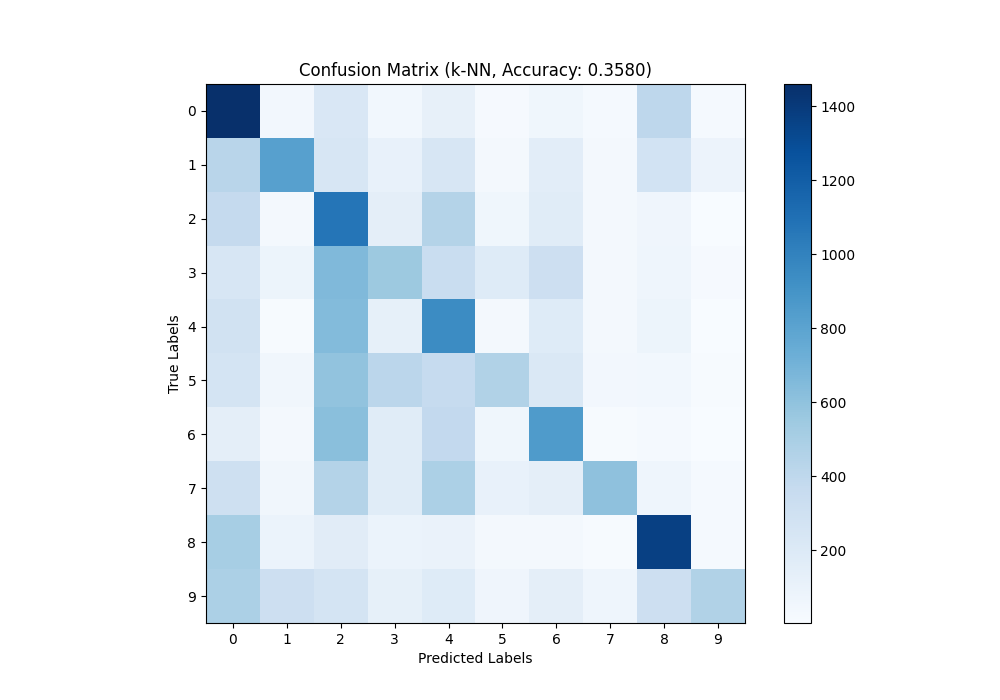
\includegraphics[width=0.5\textwidth]{grid_confusion_matrix_k-NN.png}
    \caption{Confusion Matrix for k-NN.}
    \label{fig:confusion-matrix-k-NN}
\end{figure}
\begin{figure}[H]
    \centering
    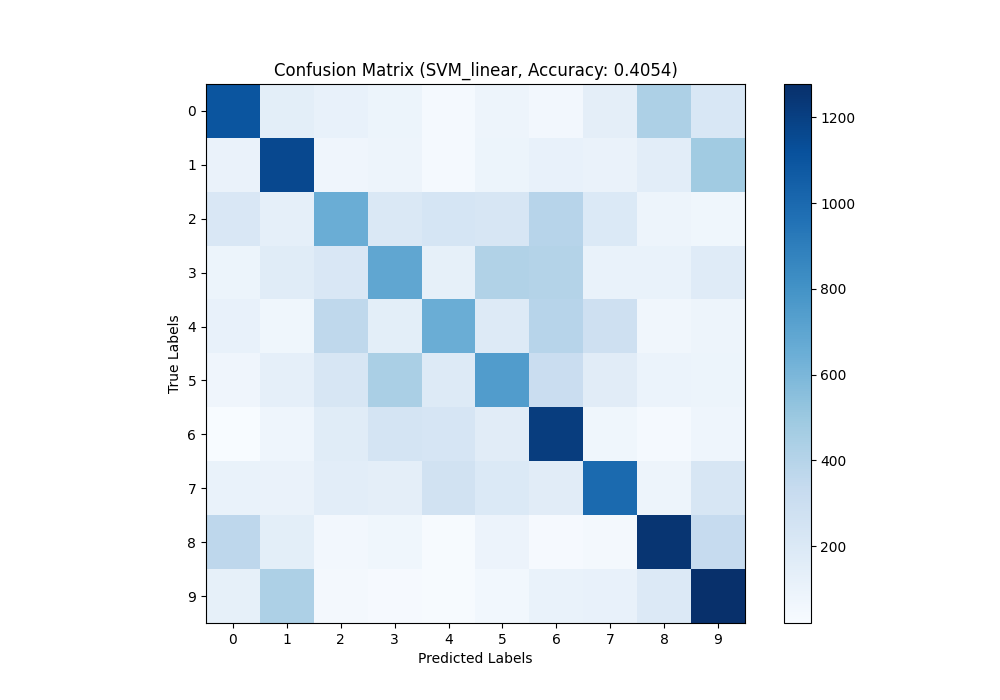
\includegraphics[width=0.5\textwidth]{grid_confusion_matrix_SVM_linear.png}
    \caption{Confusion Matrix for Linear Kernel.}
    \label{fig:confusion-matrix-linear}
\end{figure}
\begin{figure}[H]
    \centering
    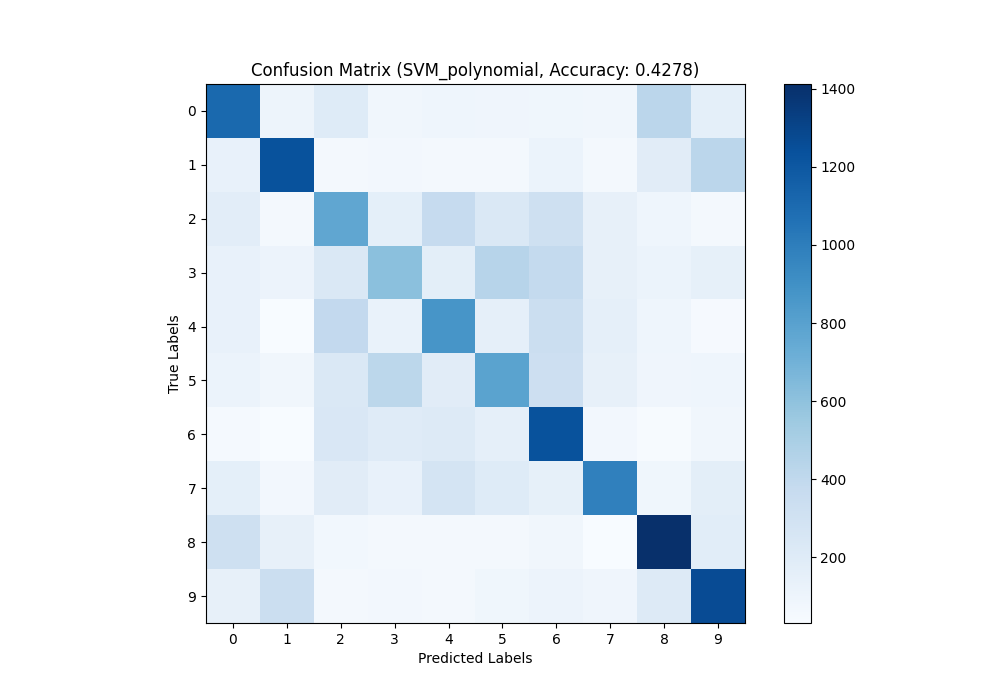
\includegraphics[width=0.5\textwidth]{grid_confusion_matrix_SVM_polynomial.png}
    \caption{Confusion Matrix for Polynomial Kernel.}
    \label{fig:confusion-matrix-polynomial}
\end{figure}
\begin{figure}[H]
    \centering
    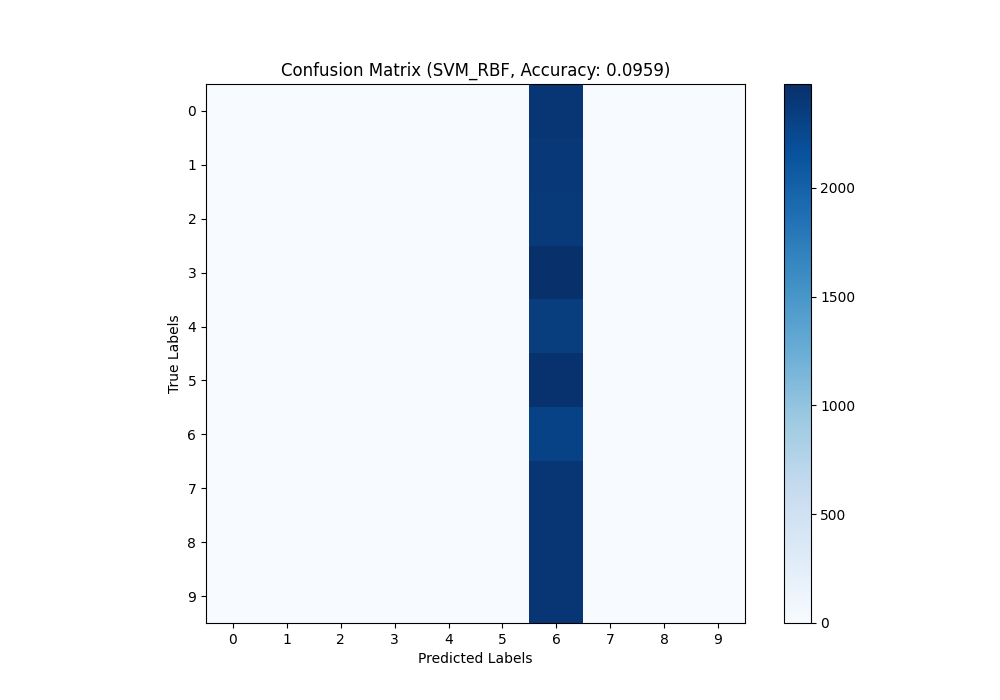
\includegraphics[width=0.5\textwidth]{grid_confusion_matrix_SVM_RBF.png}
    \caption{Confusion Matrix for RBF Kernel.}
    \label{fig:confusion-matrix-RBF}
\end{figure}
\begin{figure}[H]
    \centering
    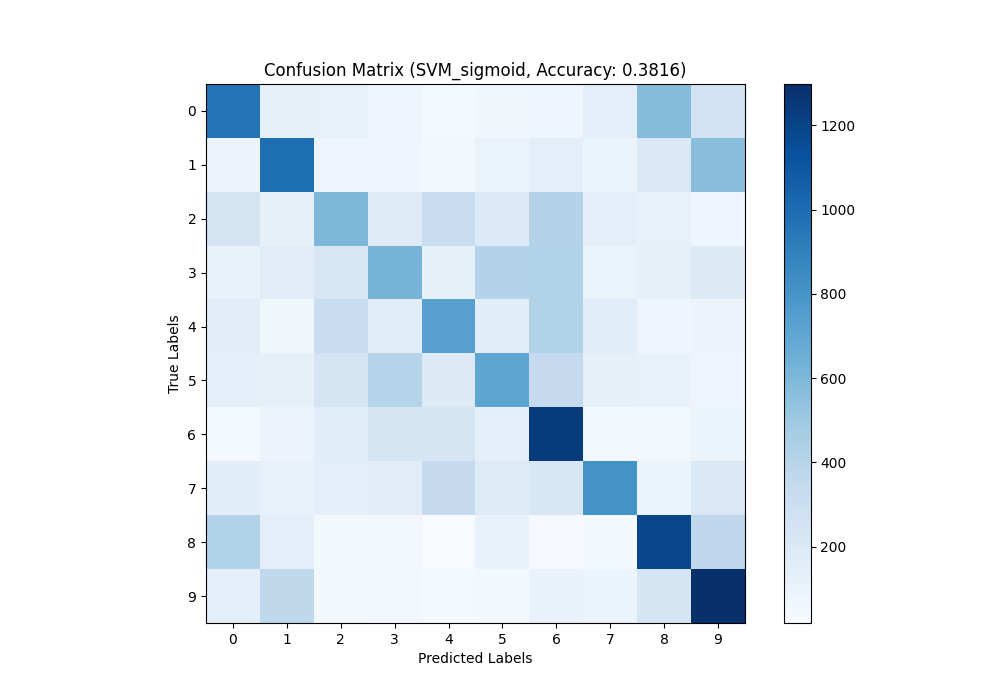
\includegraphics[width=0.5\textwidth]{grid_confusion_matrix_SVM_sigmoid.png}
    \caption{Confusion Matrix for Sigmoid Kernel.}
    \label{fig:confusion-matrix-sigmoid}
\end{figure}

\vspace{0.5cm}

\textbf{Final Thoughts:}  
The polynomial kernel worked best in terms of accuracy and training time. The linear kernel is a good choice if speed is more important. The RBF kernel might improve with better settings. That is why in section VI I demonstrated a more specific grid search with other configurations for the RBF kernel. The sigmoid kernel and k-NN were less effective, showing they are not ideal for this dataset. 

\clearpage

\section{\textbf{Grid Search and RBF Kernel Analysis}}

\subsection{\textbf{Grid Search Implementation for RBF Kernel}}
To optimize the performance of the SVM with an RBF (Radial Basis Function) kernel, a grid search was performed. This method tested combinations of $C$ and $\gamma$ values to identify the best settings. Because the previous time the grid search process took more than 16 hours to execute I now decided to go back to the 2 class implementation but using the entire dataset for them. The key steps were:

\begin{itemize}
    \item \textbf{Dataset Preparation:} 
    The CIFAR-10 dataset was filtered to include only two classes (class 0 and class 1). The maximum of samples was used for the 2 classes basicaly 12000 samples. PCA reduced the feature dimensions to 100 components to ensure faster training and testing.
    
    \item \textbf{Parameter Grid:} 
    The grid search tested combinations of regularization parameters $C = \{0.001, 0.01, 0.1, 1, 10, 100\}$ and kernel parameters $\gamma = \{0.001, 0.01, 0.1, 1, 10, 100\}$. Thus, I used an increased amount of parameters for more detailed testing.

    \item \textbf{Performance Metrics:} 
    Accuracy and F1 score were computed for each parameter combination. Additionally, the percentage of support vectors used in the training set was monitored to evaluate model efficiency.

    \item \textbf{Computational Efficiency:} 
    The time taken to train each model was recorded to compare computational costs for different parameter settings.
\end{itemize}

\vspace{0.5cm}

\subsubsection{\textbf{Results and Observations}}
The grid search results are summarized in the \texttt{rbf.txt} file, and the best parameters identified are:

\begin{itemize}
    \item \textbf{Best Parameters:} $C = 100$, $\gamma = 0.001$
    \item \textbf{Best Accuracy:} 91.60\%
    \item \textbf{Number of Support Vectors:} 3062
    \item \textbf{Total Training Time:} 362 seconds
\end{itemize}

A detailed breakdown of accuracy for all parameter combinations is shown below but the full breakdown is in \texttt{rbf.txt} file:

\begin{itemize}
    \item For $C=0.001$:
        \begin{itemize}
            \item $\gamma=0.001$: 72.75\%
            \item $\gamma=0.01$: 70.00\%
            \item Higher $\gamma$: Accuracy dropped to around 50\%.
        \end{itemize}
    \item For $C=100$:
        \begin{itemize}
            \item $\gamma=0.001$: 91.60\%
            \item $\gamma=0.01$: 91.25\%
            \item Higher $\gamma$: Accuracy dropped significantly.
        \end{itemize}
\end{itemize}

\vspace{0.5cm}

\subsubsection{\textbf{Final Model Evaluation}}
The best model was retrained using the optimal parameters ($C=100$, $\gamma=0.001$). The evaluation results were as follows:
\begin{itemize}
    \item \textbf{Accuracy:} 91.60\%
    \item \textbf{Number of Support Vectors:} 3062
    \item \textbf{Total Training Time:} 362 seconds
\end{itemize}

The results confirm that the selected parameters allow the RBF kernel to achieve high accuracy while maintaining a manageable number of support vectors, which keeps the model efficient.

\vspace{0.5cm}

\subsubsection{\textbf{Visualizing the Results}}
The accuracy for each combination of $C$ and $\gamma$ is visualized as a heatmap:

\begin{figure}[H]
    \centering
    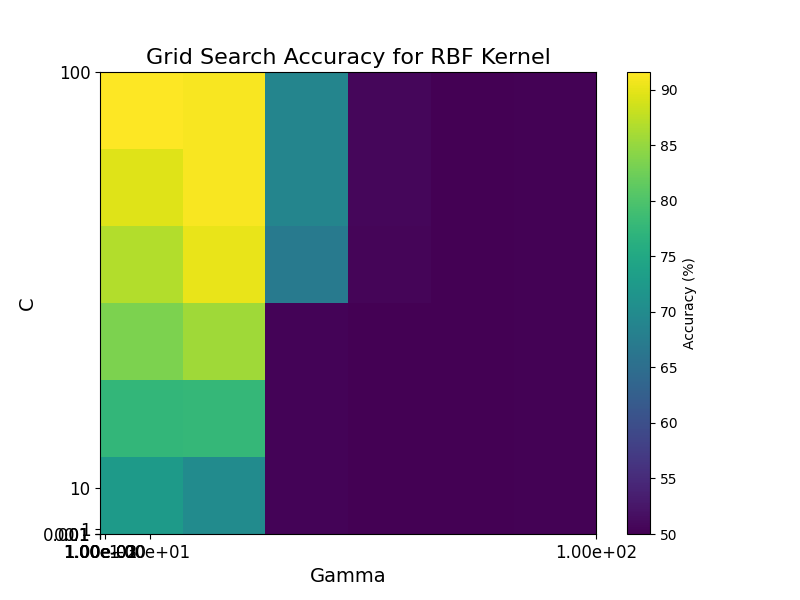
\includegraphics[width=0.5\textwidth]{grid_search_rbf_2_classes_with_pca_60000.png}
    \caption{Grid Search Accuracy for RBF Kernel.}
    \label{fig:grid-search-rbf}
\end{figure}

\vspace{0.5cm}

\textbf{Code and Results:}  
The code for this implementation is available in \texttt{RBF\_SVM.py}, and detailed results are logged in the \texttt{rbf.txt} file.

\section{\textbf{Implementation Using Sklearn SVM}}

\subsection{\textbf{Motivation for Sklearn SVM}}
After experimenting with the libsvm library, I decided to try Scikit-learn's SVM implementation for the following reasons:
\begin{itemize}
    \item Built-in functions, such as `RandomizedSearchCV`, make it easier to perform hyperparameter optimization efficiently.
    \item The ability to integrate with other Scikit-learn tools simplifies preprocessing, cross-validation, and evaluation.
\end{itemize}

\subsection{\textbf{Implementation Steps}}
The process consisted of the following key steps:

\begin{itemize}
    \item \textbf{Data Preparation:} 
   
    - The CIFAR-10 dataset was loaded, containing 50,000 training samples and 10,000 test samples, each with shape $(32 \times 32 \times 3)$. 
    
    - Images were flattened into vectors of size 3,072 (32 x 32 x 3) for compatibility with the SVM model. 
    
    - Labels corresponding to the 10 classes were extracted.

    \item \textbf{Dimensionality Reduction with PCA:}
    
    - PCA (Principal Component Analysis) was applied to the training and test sets, retaining 90\% of the variance in the data. 
    
    - This reduced the number of features from 3,072 to 99 components, which:
        \begin{itemize}
            \item Improved computational efficiency.
            \item Preserved the majority of critical information from the dataset.
        \end{itemize}

    \item \textbf{Hyperparameter Search:}
    
    - A search for optimal hyperparameters was conducted using `RandomizedSearchCV` with 2-fold cross-validation. 
    
    - The following hyperparameter ranges were tested:
        \begin{itemize}
            \item \textbf{$C$ (Regularization Parameter):} \{0.1, 1, 10, 100\}.
            \item \textbf{$\gamma$ (Kernel Coefficient):} \{'scale', 'auto', 0.001, 0.01, 0.1, 1\}.
            \item \textbf{Kernel Type:} \{'linear', 'rbf', 'poly', 'sigmoid'\}.
        \end{itemize}
    
    - A total of 5 random combinations of these parameters were tested, and the best combination was selected based on the cross-validated accuracy.

    \item \textbf{Training the Final Model:}
    
    - Using the best hyperparameters found, a final SVM model was trained on the full PCA-transformed training set.
    
    - The `OneVsOneClassifier` strategy was applied to handle the multi-class classification task.

    \item \textbf{Evaluation:}
    
    - The final model was evaluated on the test set. Key metrics, such as accuracy and prediction times, were recorded.
    
    - The first 10 predictions from the test set were saved for a qualitative review of model performance.
\end{itemize}

\subsection{\textbf{What Was Tested and Observed}}
During the implementation, the following were tested:
\begin{itemize}
    \item \textbf{Effect of PCA:}
    
    - Dimensionality reduction was tested to observe its impact on computational cost and model performance. Retaining 90\% variance with PCA reduced the feature space to 99 dimensions.
    \item \textbf{Hyperparameter Combinations:}
    
    - Various values for $C$, $\gamma$, and kernel type were tested to find the optimal configuration.
    
    - The search aimed to balance regularization ($C$) and the sensitivity of the kernel function ($\gamma$).
    \item \textbf{Kernel Comparison:}
    
    - Four kernel types were tested: Linear, RBF, Polynomial, and Sigmoid. The RBF kernel was found to outperform others significantly.
\end{itemize}

\subsection{\textbf{Results and Observations}}

\begin{itemize}
    \item \textbf{PCA Results:}
    
    - PCA reduced the feature space from 3,072 to 99 dimensions, retaining 90\% of the variance. This step reduced computational complexity without significantly impacting performance.

    \item \textbf{Hyperparameter Search Results:}
    
    - The best parameters after the search were:
        \[
        \text{{'kernel': 'rbf', 'gamma': 'auto', 'C': 100}}
        \]
    
    - The search process took 10,122.85 seconds (approximately 2.8 hours) and tested 5 random combinations of parameters.

    \item \textbf{Test Accuracy:}
    
    - Using the best parameters, the model achieved a test accuracy of 55.61\%, demonstrating moderate classification performance for the CIFAR-10 dataset.

    \item \textbf{Evaluation Time:}
    
    - Evaluation on the test set took 206.37 seconds.

    \item \textbf{Example Predictions:}
    
    - First 10 predictions on the test set were: [3, 8, 8, 0, 4, 6, 3, 6, 2, 1].
    
    - These predictions indicated the model’s ability to classify various CIFAR-10 categories, though not perfectly.
\end{itemize}

\subsection{\textbf{Visualization of Hyperparameter Search}}
The classification accuracy for each hyperparameter combination tested during the `RandomizedSearchCV` process is visualized below:

\begin{figure}[H]
    \centering
    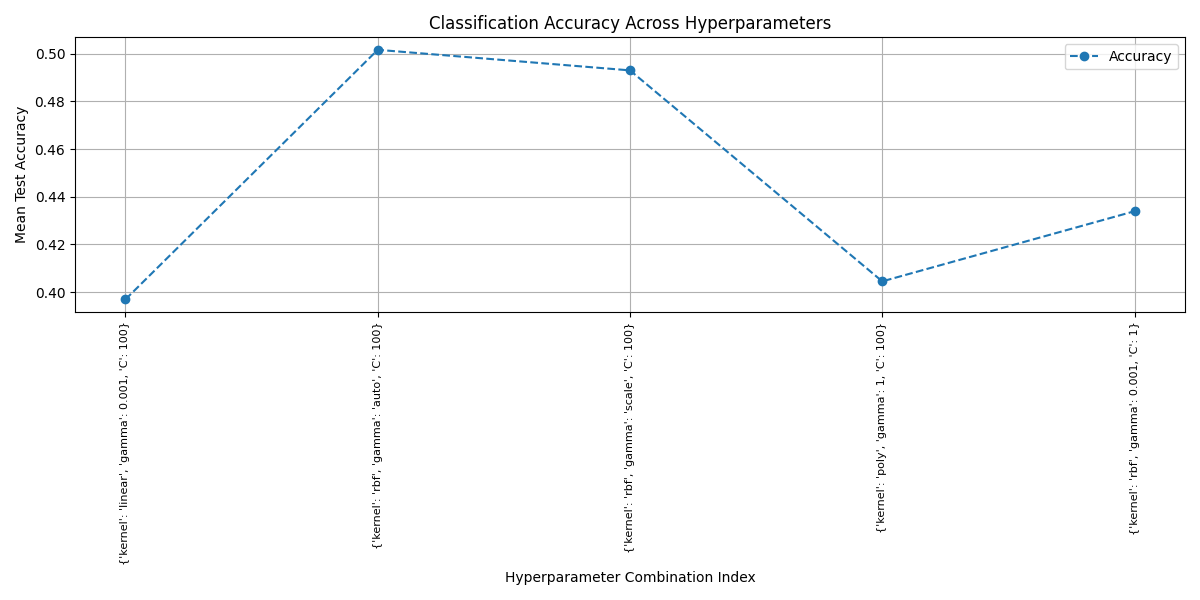
\includegraphics[width=0.5\textwidth]{classification_accuracy_hyperparameters.png}
    \caption{Classification Accuracy Across Hyperparameters}
    \label{fig:hyperparameter-accuracy}
\end{figure}

\subsection{\textbf{Conclusion}}
The implementation using Scikit-learn SVM provided a streamlined approach to training and tuning SVM models. The results showed:
\begin{itemize}
    \item \textbf{Effectiveness of PCA:} Dimensionality reduction significantly lowered computational requirements while preserving essential data features.
    \item \textbf{Optimal Parameters:} The RBF kernel with `gamma='auto'` and `C=100` achieved the best balance of accuracy and generalization.
    \item \textbf{Limitations:} Although the test accuracy of 55.61\% is moderate, further improvements could be achieved by exploring additional hyperparameters, preprocessing methods, or using a more advanced model.
\end{itemize}

The implementation code is available in the \texttt{SVC\_based.py} script, and results are logged in the \texttt{svc\_results\_with\_pca.txt} file.

\section{\textbf{Comparisons to MLP implementation}}

After comparing the train and test accuracy of the SVM models across all kernels and the k-NN algorithm, I later trained and evaluated a Multilayer Perceptron (MLP) model. Below is a detailed description of the MLP architecture, training process, and performance comparison.

\subsection{\textbf{Model Architecture}}
The MLP consists of several dense (fully connected) layers, designed to efficiently handle the CIFAR-10 classification task:
\begin{itemize}
    \item \textbf{Flatten Layer:} Converts 2D images (32x32x3) into 1D vectors for input into the dense layers.
    \item \textbf{Three Dense Layers:}
    \begin{itemize}
        \item Layer 1: 512 units with ReLU activation.
        \item Layer 2: 256 units with ReLU activation.
        \item Layer 3: 128 units with ReLU activation.
    \end{itemize}
    Each dense layer is followed by:
    \begin{itemize}
        \item \textbf{Batch Normalization:} Stabilizes learning and accelerates convergence.
        \item \textbf{Dropout:} Regularization to prevent overfitting (Dropout rates: 40\% for first two layers, 30\% for the third layer).
    \end{itemize}
    \item \textbf{Output Layer:} 10 units with softmax activation, producing probabilities for the 10 CIFAR-10 classes.
\end{itemize}

The MLP as we demonstrated in the previous assignment can learn complex patterns in the CIFAR-10 dataset.

\subsection{\textbf{Compilation and Training}}
\begin{itemize}
    \item \textbf{Optimizer:} Adam optimizer with a learning rate of 0.001, which adapts the learning rate during training for efficient convergence.
    \item \textbf{Loss Function:} Categorical Cross-Entropy, suitable for multi-class classification tasks.
    \item \textbf{Evaluation Metric:} Accuracy was used to monitor both training and validation performance.
    \item \textbf{Training Configuration:} The model was trained for 30 epochs with a batch size of 60, balancing computational efficiency and learning stability.
\end{itemize}

\subsection{\textbf{Results and Observations}}
\begin{itemize}
    \item \textbf{Train and Test Accuracy:} 
    
    - The MLP achieved a test accuracy of 44.63\%, outperforming the k-NN models and some of the SVM models like the linear and sigmoid from time to time. Although the RBF kernel SVM seems to be a lot better in accuracy since it managed a 55.61\% accuracy in the Cifar-10 dataset.
    
    - Training was way faster than grid-search-based SVMs but required more computational resources due to the large number of parameters.
    \item \textbf{Visualization:} 
    
    - Accuracy and loss curves for training and validation were plotted and saved as \texttt{training\_history\_MLP\_BEST.png}.
    
    - Correct and incorrect predictions from the test set were visualized, highlighting areas where the model performed well and struggled.
    
    - Sample predictions were saved in \texttt{sample\_predictions\_MLP\_BEST.png}.
\end{itemize}

\begin{figure}
    \centering
    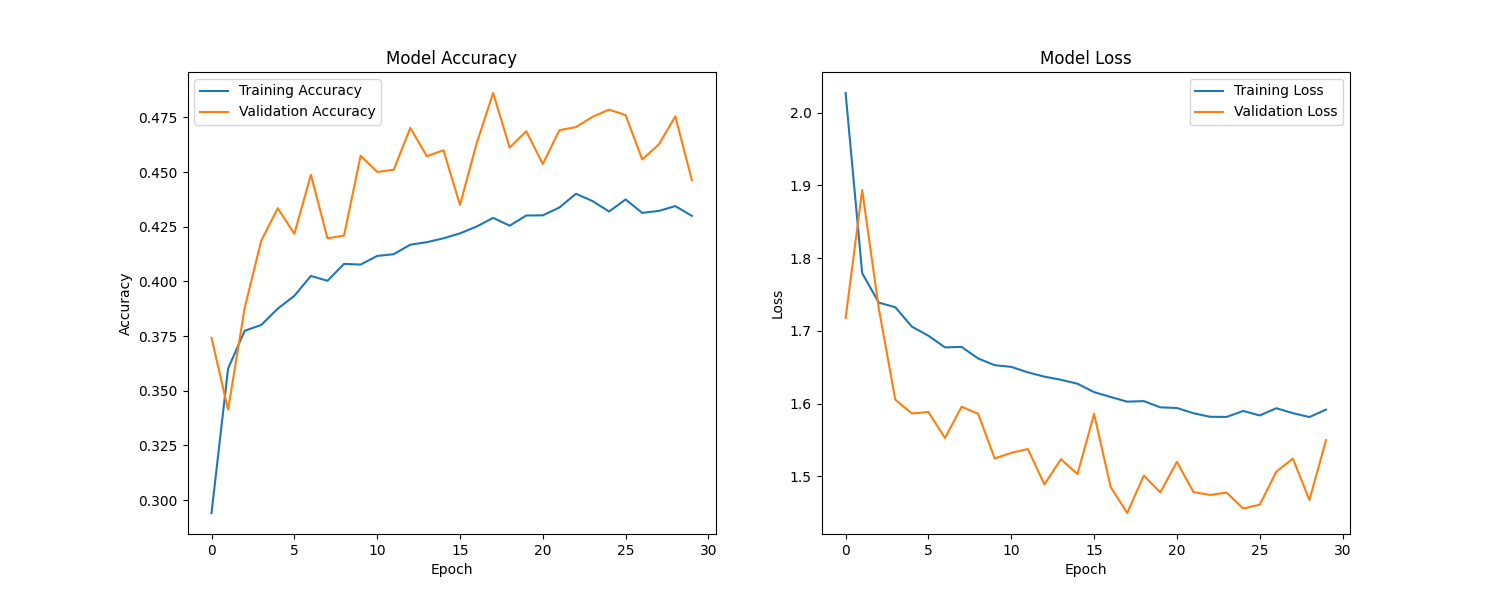
\includegraphics[width=0.5\textwidth]{training_history_MLP_BEST.png}
    \caption{MLP training history}
    \label{fig:MLP history}
\end{figure}

\begin{figure}[H]
    \centering
    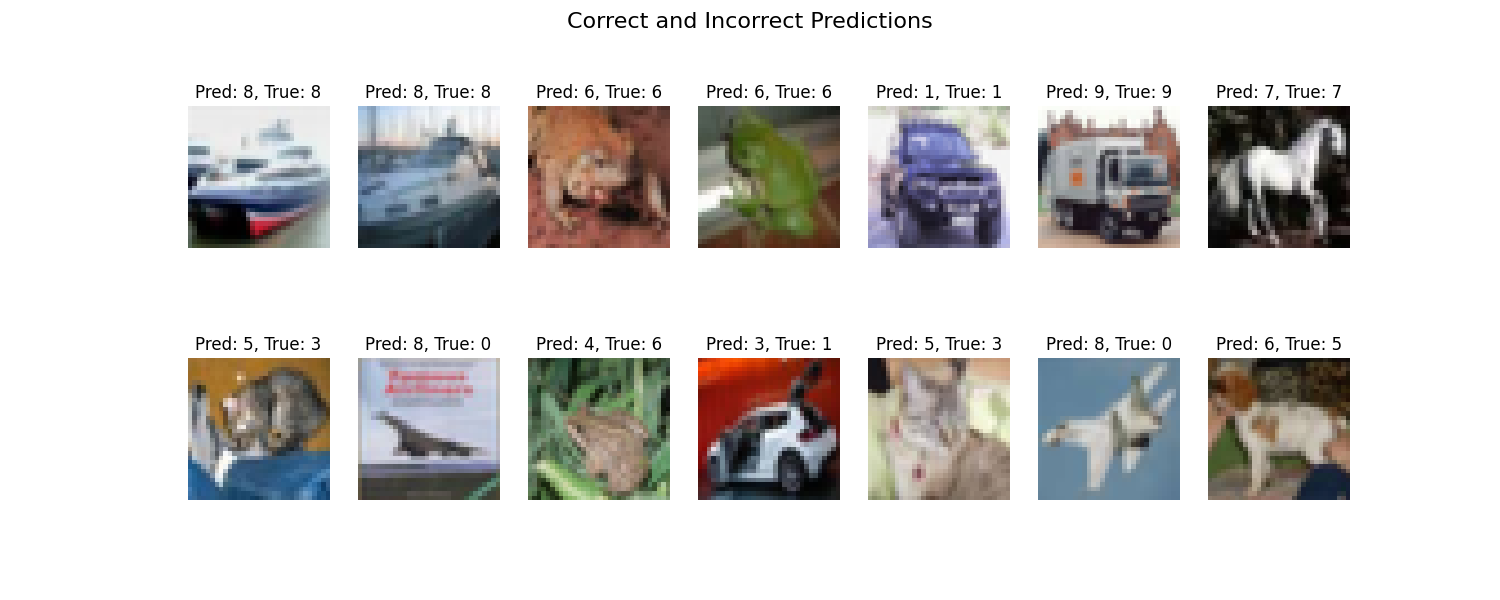
\includegraphics[width=0.5\textwidth]{sample_predictions_MLP_BEST.png}
    \caption{True and false predictions from MLP}
    \label{fig:True-False-Pred}
\end{figure}

\subsection{\textbf{Comparative Insights}}
\begin{itemize}
    \item \textbf{MLP vs. SVM:}
    
    - While SVM models required extensive hyperparameter tuning (via grid search or randomized search) to achieve reasonable accuracy, the MLP naturally handled the non-linear patterns in the data with minimal tuning. Although the Radial Basis Function Kernel SVM seems to have higher accuracy and precision than my MLP.
    
    \item \textbf{MLP vs. k-NN:}
    
    - The MLP outperformed k-NN by a significant margin, demonstrating its ability to learn complex hierarchical representations, unlike k-NN, which relies on simple distance metrics.
    \item \textbf{Regularization Benefits:}
    
    - The use of dropout and batch normalization in the MLP contributed to its improved generalization and faster convergence compared to SVMs.
\end{itemize}


\section{\textbf{References Section}}
\begin{thebibliography}{1}
\bibliographystyle{IEEEtran}
\bibitem{ref1}
https://www.ibm.com/topics/knn
\bibitem{ref2}
https://www.csie.ntu.edu.tw/~cjlin/libsvm/
\bibitem{ref3}
https://keras.io/api/layers
\bibitem{ref5}
https://scikit-learn.org/1.5/modules/svm.html
\bibitem{ref6}
https://www.cs.toronto.edu/~kriz/cifar.html
\end{thebibliography}

\end{document}


